\documentclass[a4paper]{report}
\usepackage[T1]{fontenc}
\usepackage[utf8]{inputenc}
\usepackage[english]{babel}
\usepackage{titlesec}
\usepackage{lipsum}
\usepackage{booktabs}
\usepackage{hyperref}
\usepackage{graphicx}
\usepackage{float}
\usepackage{rotating}
\usepackage[dvipsnames]{xcolor}
\usepackage{listings}
\usepackage{alloy-style}
\usepackage{geometry}
\usepackage{pdflscape}
\usepackage{caption}
\graphicspath{{./img/}}

\begin{document}

%%The two following lines remove the line "Chapter n" at the beginning of each chapter, before the title
%\titleformat{\chapter}[display]
%  {\normalfont\bfseries}{}{0pt}{\Large}
\titleformat{\chapter}[hang] 
{\normalfont\huge\bfseries}{\thechapter}{1em}{} 

\title{SafeStreets}
\author{Rosetti Nicola, Sartoni Simone, Torri Vittorio}
\date{date} %%TODO

\begin{titlepage}
\begin{figure}[t]
\centering
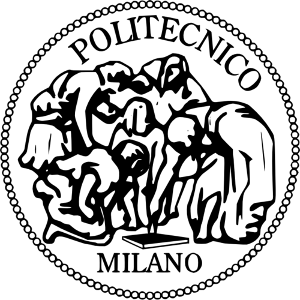
\includegraphics[width=0.3\textwidth]{Logo}
\end{figure}
\begin{center}
    \textsc{ \LARGE{Politecnico di Milano \\}}
	\textsc{ \Large {School of Industrial and Information Engineering\\ }}
	\textnormal{ \Large{Master of Science in Computer Science and Engineering\\}}
	\vspace{3mm}
	\textnormal{ \Large{Software Engineering 2 Mandatory Project\\}}
	\vspace{30mm}
	\fontsize{10mm}{7mm}\selectfont 
    \textup{Safe Streets.}\\
    \textnormal{ \LARGE{Requirement Analysis and Specification Document\\}}
\end{center}

\vspace{18mm}

\begin{center}
    \textnormal{\large{\bf Authors:\\}}
	{\large Rosetti Nicola \\ Sartoni Simone \\ Torri Vittorio }
	\fontsize{10mm}{5mm}\selectfont 
\end{center}
\vspace{15mm}

\centering{\large{
Academic Year 2019/2020 \\
\vspace{10mm}
Milano, 10/11/2019 \\
\vspace{2mm}
Version 1.0 
}}

\end{titlepage}

\newgeometry{top=3cm}
\tableofcontents
\listoffigures
\begingroup
\let\clearpage\relax %avoid to put it on a new page
\listoftables
\endgroup
\restoregeometry
\chapter{Introduction}
\section{Scope}
SafeStreets is an application meant to provide a mechanism to more efficiently detect parking violations and to try to make streets safer. This is meant both for normal people and for municipality agents. 
The application domain concerns different types of world phenomena, shared phenomena and machine phenomena. \\
We can identify the following world phenomena:
\begin{itemize}
\item {[W1]} \label{W1}A car is illegally parked 
\item {[W2]} \label{W2}An accident occurs
\item {[W3]} \label{W3}An intervention is performed to make the roads safer
\end{itemize} 
the following shared phenomena controlled by the world and observed by the machine:
\begin{itemize}
\item {[S1]} A violation report is sent by a user
\item {[S2]} An accident report is provided by the municipality system
\item {[S3]} New information about issued tickets are provided by the municipality system
\end{itemize}
and the following shared phenomena controlled by the machine and observed by the world:
\begin{itemize}
\item {[S4]} A traffic ticket is emitted by an agent, exploiting the municipality system, after a report analysis
\item {[S5]} An agent is sent to verify the correctness of a violation report
\item {[S6]} A suggestion for a safety improvement on streets is made available
\end{itemize}

\section{Purpose}
The system is characterized by the following goals, distinguished by the function provided:
\begin{itemize}
\item {Violations and tickets function:}

\begin{itemize}
\phantomsection
\item{[G1]} \label{G1}People must be allowed to report parking violations (missing parking disk, not paid parking meter, illegally parked vehicles).
\phantomsection
\item {[G2]} \label{G2}Municipality agents must be notified about reports of potential violations in their area of interest, which can be possibly used to generate traffic tickets.	
\end{itemize}

\item {Statistic functions:}
\begin{itemize}
\phantomsection
\item  {[G3]} \label{G3}People must be allowed to retrieve information about streets or areas with the highest frequency of violations.
\phantomsection
\item  {[G4]} \label{G4}People must be able to retrieve statistics and trends about the accidents correlated to the parking violations, the effectiveness of SafeStreets initiatives and the issuing of traffic tickets.
\phantomsection
\item  {[G5]} \label{G5}Municipality supervisors must be able to retrieve data about the vehicles with the highest number of violations.
\phantomsection
\item  {[G6]} \label{G6}Municipalities must be suggested for possible interventions about the mostly unsafe areas.
\end{itemize}
\end{itemize}

In the following table is shown which world and shared phenoma are involved for each goal.
\begin{table}[H]  
  \centering
  \begin{tabular}{|c|c|c|c|c|c|c|c|c|c|}
    \cline{2-10}
    \multicolumn{1}{c|}{} & W1 & W2 & W3 & S1 & S2 & S3 & S4 & S5 & S6 \\ \hline
    G1 & X &   &   & X &   &   &   &   &   \\ \hline
    G2 & X &   &   & X &   &   & X & X &   \\ \hline
    G3 & X &   &   & X &   & X &   &   &   \\ \hline
    G4 & X & X &   & X & X & X & X &   &   \\ \hline
    G5 & X &   &   &   &   & X & X &   &   \\ \hline
    G6 &   &   & X &   &   &   &   &   & X \\ \hline
  \end{tabular}
  \caption{Correspondence between goals and world and shared phenoma}
\end{table}

\section{Definitions, acronyms and abbreviations}
\begin{itemize}
\item \textit{GPS}: Global Positioning System
\item \textit{HTTPS}: HyperText Transmission Protocol over SSL
\item \textit{IDS}: Intrusion Detection System
\end{itemize}
\section{Revision history}
\begin{itemize}
\item 10-11-2019 Version 1.0
\end{itemize}
\section{Reference documents}
\begin{itemize}
\item Assignment Document "SafeStreets Mandatory Project Assignment.pdf"
\end{itemize}
\section{Document structure}

The document consists of 4 chapters:
\\ 
\\
\textbf{Chapter 1}: In this chapter is presented basically the domain of the application, taking into consideration all the world and shared phenomena that the application observes and/or controls. The scope of the application is specified, listing all the goals.
It also contains additional information to make the reading of the document more understandable.\\ \\
\textbf{Chapter 2}: In this chapter the application itself is taken into consideration, concerning its functions and the potential stakeholders that actually will use it. Considering users and the world in which they act, all the assumptions made on the domain are listed. A series of UML diagrams (Class and State diagrams) are then presented to help understanding how the application should work in terms of entities involved and functionalities.\\ \\
\textbf{Chapter 3}: 
In this chapter the application behavior is described: at first some scenarios are identified and then some UML diagrams (sequence and use cases diagrams) are provided, with a detailed analysis of the use cases; at last by specifying requirements in terms of :
\begin{itemize}
\item functional requirements;
\item non-functional requirements;
\item interface requirements.\\ \\
\end{itemize}
\textbf{Chapter 4}: In the last chapter a brief but concise and effective formal analysis of the problem is presented using alloys. Some requirements and domain assumptions are formally specified and their consistency is verified, with the help of the Alloy tool.
\\

\chapter{Overall Description}
\section{Product perspective}
In figure \ref{fig:class-diagram} is reported an \textit{UML Class Diagram} which represents the domain of the application with main concepts and data involved, including their relationships.\\
Not all classes will necessary become effective classes in the implementation (e.g. the \textit{Visitor} class).
Some data appear to be duplicated in the \textit{TrafficTicket} class but it needs to be considered the fact that the application will receive also data about traffic tickets which have not been issued as a consequence of a SafeStreets report, but instead have been independently issued by the local police in their traditional control activities. They are necessary to correctly build statistics and they need to include data which are already present in the corresponding report, when it exists.\\
For what concerns the \textit{Accidents} here it has been supposed a representation for all types of accidents, coming from the municipality data, with a specified type for accidents related to bad parked cars.\\
For what concerns statistics here there is a double hierarchy: a division between area and street statistics and a division between public and the reserved (i.e. only for municipality supervisors) ones. As it will be explained later, the system allows users to see the areas or streets with the most frequent violations or with the better improvements and similar other classifications, but here, in the Class Diagram, only the basic data which allow to build this more complex statistics are represented, both for simplicity and because probably other classifications will be calculated on demand, avoiding to maintain a copy constantly updated.  \\
In figure \ref{fig:state-diagram1} is reported an \textit{UML State Diagram} to clearly represent the state evolution of a \textit{ViolationReport}, which is the main object which change its state in the time, while the other ones do not present significant evolutions from this point of view.

\newgeometry{top=0.1cm}
\begin{figure}[p]
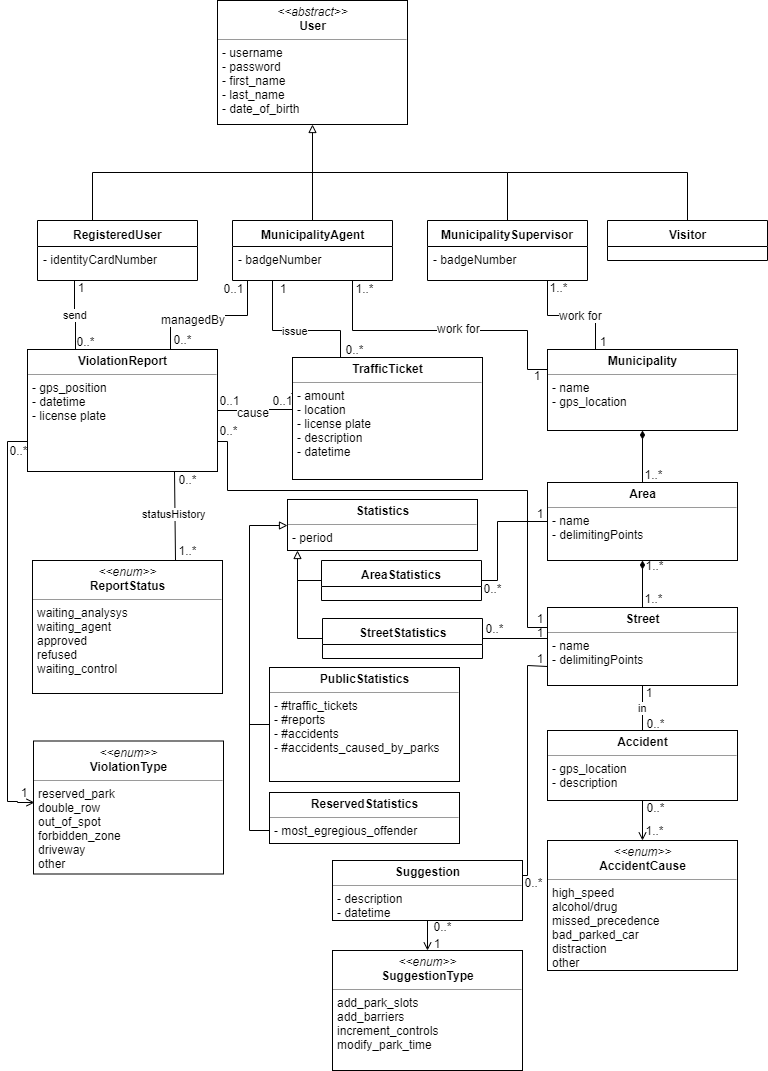
\includegraphics[width=\textwidth]{ClassDiagram2}
\caption{UML Class Diagram}
\label{fig:class-diagram}
\end{figure}
\restoregeometry

\begin{figure}[hp]
\centering
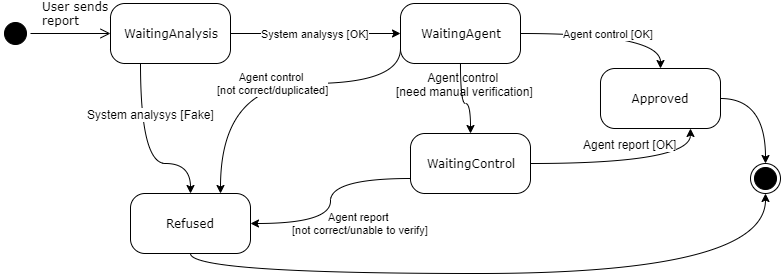
\includegraphics[width=\textwidth]{StateReport2}
\caption{UML State Diagram for ViolationReport}
\label{fig:state-diagram1}
\end{figure}



\section{Product functions}
In this part are underlined the main functions offered by SafeStreets, divided by the users that can actually have access to them.

\subsection{Visitor}

\subsubsection{Registering to the application}

The system offers the possibility to Visitors to register and actually become users of the application. When registering the visitor needs to provide his name, surname, birthdate, fiscal code and identity card number. They are mandatory so if some of them is not provided then the registration process fails.
 
\subsection{AuthenticatedUser}

\subsubsection{Reporting a violation}
This is the most important function offered by SafeStreets. This function allows Users, when logged in, to report a potential violation that has occured in the streets. 
They can achieve that by inserting some mandatory data. When reporting a violation, a user must insert the type of violation that has been detected ( missing park disk, car illegally parked in the bike lane, car illegally parked in some reserved parking spot, not paid parking disk).
Subsequently, the user must provide at least one picture of the violation. Through the pictures, the user should provide clear evidence of the violation and the vehicle involved (in particular the license plate) before sending the report for a verification to the server. The user can help recognition providing the license plate of the vehicle as plain text. Before sending the report, the application attaches to it the current position of the User (using GPS position) and date and time of the report.

\subsection{Municipality agent}
\label{sub-agentfun}
\subsubsection{Violation checking}
After logging in as a municipality agent, the system notifies the agent about all the current not resolved reported violations. The agent can visualize individually each report, starting from the oldest one in terms of date and time, checking if the report corresponds to an actual violation. He can either directly emit a traffic ticket or send an agent on the street to check and eventually emit the ticket.  If he decides to send an agent to verify the report he can put it on hold and take it back later from the "On hold" queue. It can also refuse the report if it is duplicated or if he is sure that is not a real violation. In this case he can also access the report author's data. He can then proceed and check the next report on the queue, if present.\\
Additionally, when he is logged, the agent is notified of new incoming reports.\\
Reports which are automatically rejected by the system controls are shown to the agents as rejected and they can check them and obtain the author's data.

\subsection{Municipality supervisor}

\subsubsection{Suggesting possible solutions} 
This function consists of a task periodically executed by the system (once a month) which tries to analyze reported violations, issued tickets, accidents information and data about the streets network coming from the municipality to suggest possible interventions to increase the safety (e.g. add barriers, create new park spots, increase the allowed parking time, send more agents in a certain area in certain hours...). When the system finds new suggestions for certain streets it sends them to the municipality supervisors.

\subsubsection{Consult reserved statistics}
This function allows logged in municipality supervisors to retrieve information about the vehicles with the highest number of violations in a selected area/street. The area/street must be in the supervisor's area of competence.

\subsection{Municipality agents and supervisors}
\subsubsection{Authority agent registering}
Differently from the function previously explained and meant for normal Users, this function is only meant for Municipality agents or supervisors. Each agent which needs to be officially registered needs to provide his name, surname, birthdate, rank and badge number. After providing a password, the registration is sent for a verification to the municipality service and completed if the data inserted is correct. An ID code is then given to the agent to be uniquely identified.

\subsection{Everyone} 

\subsubsection{Consulting statistics}
This function allows visitors, users, municipality agents or supervisors to retrieve information about the streets and areas with the highest frequency of violations; it is possible to retrieve statistics and trends about the accidents correlated to the parking violations, the effectiveness of SafeStreets initiatives and the issuing of traffic tickets. The information provided must be mined by the system from the reported violations, crossed with information from municipality. The system must not allow users to see confidential data about other people; it must allow the user to choose a topic: areas/streets with most accidents, areas/streets with the highest number of traffic tickets issued or areas/streets where there have been the best improvements or he can select a specific street or area for which he want to see the data. In the end the system must show to the user the information about the topic selected.



\section{User characteristics}
The users of the service are the following:
\begin{itemize}
\item \textit{Visitor}: a non-logged user which can only consult statistics about areas with the highest frequency of violations, highest rate of accidents related to the violations, traffic tickets issued and safety improvements. 
\item \textit{Authenticated User}: an identified user which, in addition to the \textit{visitor}, can report a parking violation, sending the details to the municipality authorities.
\item \textit{Municipality agent}: an agent of the local police which is notified about the violation reports for his municipality and can manage them as described in \hyperref[sub-agentfun]{\textit{Violation checking} function.}
\item \textit{Municipality supervisor}: he has a full access to the application data, including all statistics and the suggestions to improve safety in the most dangerous areas.
\end{itemize}
\section{Assumptions, dependencies and constraints}
\subsection{Dependencies and constraints}
\label{SS-Dep&Const} 
The presence of some services provided by the municipalities is necessary to make all SafeStreets functions operative. In particular the following services are requested:
\begin{itemize}
\item \textit{Identity Card Check}: allows to retrieve data of a person given its identity card number.  It's request for a strong user authentication.
\item \textit{Statistics Information}: return information about the accidents occurred in the municipality streets and about the parking violations traffic tickets issued outside the SafeStreets system, with position and causes.
\item \textit{Road Network Information}: allows to retrieve information about the streets characteristics, such as park slots, park time, sidewalks, barriers.
\item \textit{Traffic Ticket Issue}: allows to send traffic tickets to a certain person by a certain agent
\item \textit{Agents Identity Check}: allows to check the identity of a registering agent given his personal data, including his badge number. 
\end{itemize}
\subsection{Domain Assumptions}
\label{subsec:domain-ass} 
Here are shown the domain assumptions:
\begin{itemize}
\item{[D1]} \label{D1} GPS is always precise, giving the position with an error of maximum 5 meters.
\item{[D2]} \label{D2}Smartphone cameras have enough resolution to enable recognizing algorithms
\item{[D3]} \label{D3}Every municipality which exploits the SafeStreets services has defined some areas in which the city is divided, eventually overlapped, and every street of the city is at least in one area (in the worst case the entire city is a single area)
\item{[D4]} \label{D41}The identity card is unique for each person.
\item{[D5]} \label{D5}Each person has only one identity card.
\item{[D6]} \label{D6}The \textit{Traffic Tickets Issue} service of the municipalities always issue traffic tickets if it receives the correct information and if it is available (i.e. it is not in a downtime moment).
\item{[D7]} \label{D7}Every registered municipality agent has a unique ID (badge number) inside its municipality.
\item{[D8]} \label{D8}Every municipality that uses SafeStreets has at least one Agent and one Supervisor that are in charge for managing SafeStreets services.
\item{[D9]} \label{D9}Every agent and supervisor works for exactly one municipality.
\end{itemize}

\chapter{Specific Requirements}
\section{Scenarios identification} 
Here are presented possible scenarios for the different users of the system.\\ \\
\textbf{Scenario 1. Report of a violation}\\
\\
Mark is a man in his thirties. He’s an employee at Esselunga supermarkets. One day, walking down the main street of his city he finds a car parked illegally in the middle of the bike lane. Mark is registered in the application SafeStreets. He takes out his smartphone and opens the application. After writing his credentials and logging in, he clicks the button “Report a violation” in the home page. He inserts the type of violation, so in this case he just writes “car illegally parked in bike lane”, and takes three different pictures of the car: one of the front of the car, clearly showing the license plate; the second showing the entire car and, in the background, the signal of bike lane; the third one highlighting important elements of the streets where the potential violation occurred, to help the matching of the photo with the GPS position of the user. He then confirms clicking on the “Confirm” button. The potential violation is now sent to the server for a verification. Finally, he closes the application and continues his walk.
\\
\\ 
\textbf{Scenario 2. The agent receives a notification and issues a traffic ticket}\\
\\
Lukas is a municipality agent that is working as usual at his desk and has the SafeStreets Web app opened in the background on his PC. While checking his papers he receives a notification from the SafeStreets. He opens the window of the app and finds that a new report has been made about a violation. Lukas clicks on the row linked to the new violation. He observes that the violation has been reported by a certain Gianluca Verdi. The pictures of the report clearly show the vehicle that has made the violation (not paid parking meter), his license plate and the place where the violation occurred. There is now enough evidence that allows Lukas to issue a traffic ticket to the owner of the vehicle.
\\
\\
\textbf{Scenario 3. A policeman receives a notification and send an agent to control because the picture is not clear}\\
\\
Laura is a municipality agent that has just started her new day at work. She works in Milan's police station. She starts her PC at her desk, opens Internet Browser and search for SafeStreets Web App. After logging in, the reported violation queue is filled with 10 notifications of new potential violations reported. She opens the first one and she discovers that the system wasn't able to correctly identify the vehicle involved and the user hasn't inserted an existing license plate. She checks the pictures but she can't find out what is written on the license plate. She tells his supervisor the problem, in order to send an agent to directly check in the place of the supposed violation (based on the GPS position sent by the user) and, possibly, to issue a traffic ticket.
\\
\\
\textbf{Scenario 4. A user checks for unsafe streets in his zone}\\
\\
Bob is a curious user that has the SafeStreets application installed in his iPhone 8 but is not registered in the SafeStreets database. One day, he witnesses an accident in the streets while driving his car, where a car hits a biker during a parking manoeuvre on a runs over a biker correctly biking in his bike lane.
As he goes home, he’s curious about the most dangerous and unsafe areas and streets in his city and he wants to see if the street where he saw the accident is one of them. He opens the SafeStreets application and clicks the button “Check statistics in a city”. After this, a new page opens in which Bob clicks on the “Check for most dangerous areas/streets”. The last click he does is on the “Search for a city using your GPS position” button. Now the screen shows a map with highlighted the most unsafe areas (with most accidents) in his city. Bob selects then the area in which he is interested in and he sees which are the most dangerous streets in the area. Bob discovers that the street he was searching for is the most dangerous one. Finally, Bob closes the application.
\\
\\
\textbf{Scenario 5. Needs to travel and searches for safe places for a car}\\
\\
Marie is a woman who often travels for work. She typically travels by car. She lives in Milan and this week she needs to go to Turin. He wants to know where she can safely park the car and take an hotel reservation. Before searching for an hotel, she takes out her Huawei and opens the SafeStreets application. She clicks the button “Check statistics in a city”. After this, a new page opens in which Bob clicks on the “Check for most dangerous areas/streets”. The last click he does is on the “Select a city you want” button. She chooses “Turin” among all the possible ones. Now she can use found information to look for safe zones near her workplace.
\\ 
\\
\textbf{Scenario 6. New intervention suggestion for an unsafe street}\\
\\
Marco is a local police supervisor in the municipality of Varese. He logins in the SafeStreets application and he sees a notification about a suggestion for an intervention to improve safety. He opens it and he reads that in Via Roma there have been a lot of reports and consequent tickets in the last months due to cars parked on the sidewalk. The system is suggesting to add barriers to prevent cars from going on the sidewalk. This seems a good suggestion for him, he will discuss it with the competent municipality sector. 
\\
\\
\textbf{Scenario 7. The user registers to the application}\\
\\
Luke and Walter are two close friends. Luke doesn’t know about SafeStreets application while Walter is a regular registered user of it. One day, Walter and Luke are walking down a road. Walter notices a potential violation and stops. He takes out his phone and opens the SafeStreets application. Luke asks Walter what he’s doing and Walter explains what SafeStreets is. Walter is pretty convincing and makes Luke install the application. Luke learns that to report violations he needs to register. So, he starts the process of registration providing his name, surname, birthdate, fiscal code and number of the identity card. After this, he creates his own unique username and the password. On screen, Luke sees that the registration has been successful. 
\\
\\
\textbf{Scenario 8. A supervisor wants to check see what areas are registering improvements since the municipality has started to use SafeStreets}\\
\\
Giulio is a local police supervisor in the municipality of Milan. It’s six months since they have started to use the SafeStreets application to receive report from citizens about parking violations and he want to check what benefits it has brought. He opens the web application, he logins inserting his credentials and he clicks on Improvements under the Statistics section. Here he can see what streets have seen the best reduces in the number of issued tickets. He sees that a lot of central zones have seen reductions from 20 to 50 percent, while in the peripheral areas the numbers are much less substantial. He is happy because of this result, but he wants to improve it and he thinks to start a marketing campaign to encourage more people to use the application, especially in the peripherals. 
\\ 
\\
\phantomsection %to link back SLANDER note
\label{use:slander}\textbf{Scenario 9. Marco wants to make a joke to a friend and send a fake report}\\
\\
Marco and Luigi are two very close friends. One day Marco decides it's time to make a very not funny joke to his friend and he decides to use the SafeStreets application to make him receive a traffic ticket. He finds an illegally parked car, he photographs it and then he tries to modify the license plate in the photo with Luigi's car license plate. He sends the report with the modified photo thinking about the face of Luigi when he will receive the ticket. 
Some weeks later he receives a letter from the judicial authority stating that they have started a criminal proceeding against him for the crime of slander (see \hyperref[ref:slander]{\textit{[SLANDER]}}).
Probably he won't do it another time. 
\\ 
\\
\textbf{Scenario 10. A municipality agent registers to the application}\\
\\
Ben is a new local police agent in the municipality of Bologna hired only two days ago and his supervisor says him that he has to register to the SafeStreets application. So Ben open the already installed application from his Computer and clicks on the "Register" button on the homepage. He inserts his name, surname, birthdate, rank and badge number, then he chooses his password, equal to "LKJVC89", and confirm the inputs. After the registration is processed, Ben receives his unique ID and is returned to the home page. He can now properly work.

\section{UML diagrams analysis}

\subsection{Use case diagram}
In figure \ref{fig:useCases} is report the UML Use Case Diagram.
\begin{figure}[hpt]
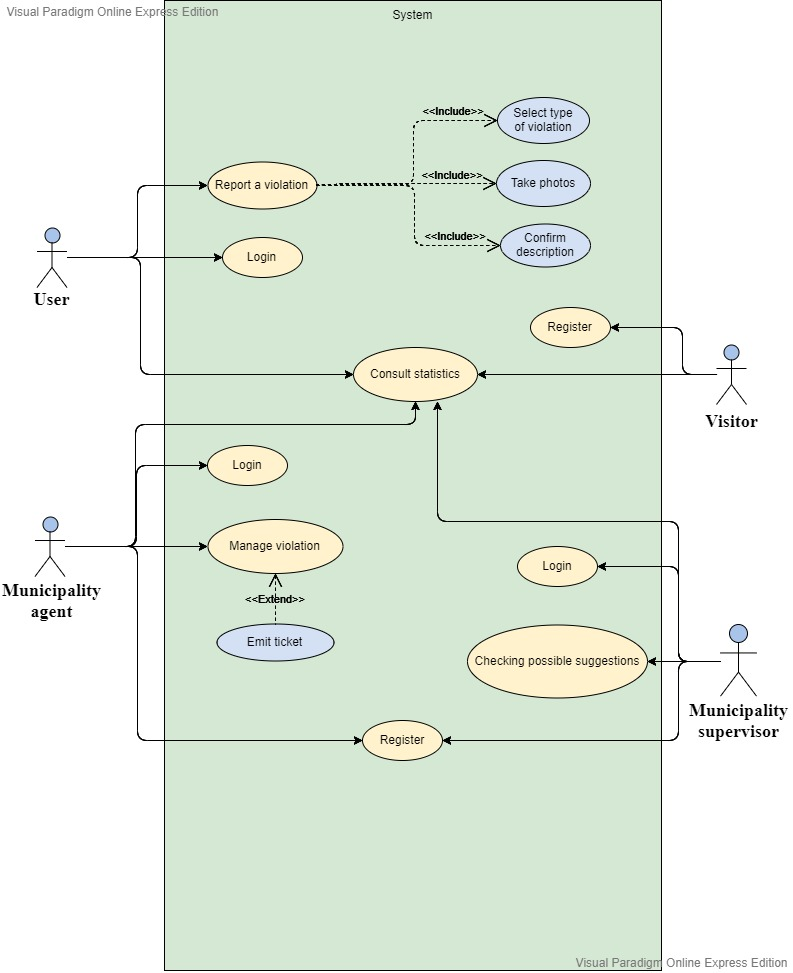
\includegraphics[width=\textwidth]{UseCaseDiagram}
\caption{Use Case Diagram}
\label{fig:useCases}
\end{figure}

\subsection{Use case identification}
In this section the various use cases present in the use case diagram and derived from the scenarios previously described are illustrated in detail.\\ \\
\phantomsection
\textbf{1. User logs in}\label{uc:1}
\\
\\
Actors: User\\ \\
Entry condition: 
\begin{itemize}
\item The User needs to have the application opened
\end{itemize}
Flow of events:
\begin{itemize}
\item The User clicks on the login button
\item The user input his username (ID) and his password
\item The user clicks on the “confirm” button
\item The system redirects the taxi driver to his personal homepage
\end{itemize}
Exit conditions: 
\begin{itemize}
\item The user is successfully redirected to his personal homepage
\end{itemize}
Exceptions: 
\begin{itemize}
\item The code and password provided by the user are not correct. In this case, the system does not redirect the user to his personal homepage but notifies him that an error has been made and allows to input his code and password again
\end{itemize}
\phantomsection
\textbf{2. User reports a violation}\label{uc:2} \\ \\
Actors: Authenticated User\\ \\
Entry condition:
\begin{itemize}
 \item The user must be logged in and on his personal homepage.
 \end{itemize}
Flow of events:
 \begin{itemize}
\item The user input clicks on the “Report violation” button.
\item The user sets the “type of violation” button to a desired value, chosen from a choice list.
\item The user clicks on the “take photos” button and complete the operation.
\item The user eventually fills the form “license plate”.
\item The user clicks on the “confirm” button and is redirected to his personal home page.
\end{itemize}
Exit conditions:
\begin{itemize}
\item The system checks the report and manages it, checking if images are corrupted and eventually forwarding the report to the municipality agent.
\item	Before confirming, the User clicks on the "Back” button and cancels the current report. Pictures are cancelled too. 
\end{itemize}
Exceptions: \\
There are no exceptions for this use case. 
\\
\\
\phantomsection
\textbf{3. Agent or supervisor registers}\label{uc:3}
\\
\\
Actors: Municipality agent or Municipality supervisor \\ \\
Entry condition:
\begin{itemize}
\item the agent or supervisor needs to have the Web App opened.
\end{itemize}
Flow of events:
\begin{itemize}
\item The agent/supervisor opens the application and arrives at the homepage.
\item The agent/supervisor clicks on the "Register" button.
\item The agent/supervisor input his name, surname, birthdate, rank and badge number.
\item The agent/supervisor input his choosen password.
\item The agent/supervisor clicks on the "Complete Registration" button.
\item The system processes the registration and send information to the Municipality Service.
\item The system notify the agent/supervisor about his new Unique Identifier (ID) and suggest to remember it. 
\item The agent/supervisor clicks on the "Understood" button.
\item The system redirects the agent/supervisor to login page.
\end{itemize}
Exit conditions:
\begin{itemize}
\item The agent/supervisor is successfully redirected to login page.
 \end{itemize}
Exceptions: 
 \begin{itemize}
 \item The name, surname, birthdate, rank and badge number furnished by the agent are not found by the municipality service. In this case, the system does not redirect the agent/supervisor to the login page, but notifies him that an error has been made and allows to insert the data again.
\end{itemize}
\phantomsection
\textbf{4. Agent or supervisor logs in }\label{uc:4}
\\
\\
Actors: Municipality agent or Municipality supervisor \\ \\
Entry condition:
\begin{itemize}
\item the agent/supervisor needs to have the Web App opened.
\end{itemize}
Flow of events:
\begin{itemize}
\item The agent/supervisor opens the application and arrives at the homepage.
\item The agent/supervisor clicks on the “Login” button.
\item The agent/supervisor input his username and password.
\item	The agent/supervisor clicks on the log in button.
\item	The system redirects the agent/supervisor to his personal page.
\end{itemize}
Exit conditions:
\begin{itemize}
\item The agent/supervisor is successfully redirected to his personal page.
 \end{itemize}
Exceptions: 
 \begin{itemize}
 \item The username and password furnished by the agent/supervisor are not correct. In this case, the system does not redirect the agent/supervisor to his personal page, but notifies him that an error has been made and allows to input his username and password again.
\end{itemize}
\phantomsection
\textbf{5. Checking statistics}\label{uc:5}
\\ \\
Actors: everyone \\ \\
Entry condition: 
\begin{itemize}
\item The user needs to have the application opened
\end{itemize}
Flow of events:
\begin{itemize}
\item The user clicks on the Checking statistics button in the main page
\item The user chooses to get statistics either from his city or from another one
\item The user selects the type of statistics: data about a specific street or area, or a classification of streets or area on the base of the number of reports,tickets,accidents or increase/reduction in these values.
\item After checking, user presses the Back button to return to the home page
\item The system asks the user if he is sure to exit with a “Yes” or “No” choice
\item The user presses the button he wants, confirming his choice
\end{itemize}
Exit conditions:
\begin{itemize}
\item User is successfully brought back to the home page
\end{itemize}
Exceptions: \\There are no exception in this case
\\ \\
\phantomsection
\textbf{6. Supervisor checks potential intervention}\label{uc:6}
\\ \\
Actors: Supervisor \\ \\
Entry condition: 
\begin{itemize}
\item The supervisor must be logged in. Possibly he have received a notification about a new available suggestion. 
\end{itemize}
Flow of events:
\begin{itemize}
\item The supervisor clicks on the “Recent Suggestions” button or clicks on the new suggestion notification.
\item The system redirects the supervisor to a page where he can see the list of suggestions from the most recent to the oldest
\item The supervisor chooses a suggestion.
\item The system shows the supervisor the whole text of the suggestion.
\item The supervisor clicks the “Done” button and is redirected again to his homepage.
\end{itemize}
Exit conditions:
\begin{itemize}
\item The supervisor is successfully brought back to his personal home page.
\end{itemize}
Exceptions:
\begin{itemize}
\item There are no recent suggestions, so the system notifies the supervisor about this exception. The system redirect the supervisor to his personal page.
\end{itemize}
\phantomsection
\textbf{7. Agent checks a notified violation}\label{uc:7}
\\ \\
Actor: Municipality Agent \\ \\
Entry condition: 	
\begin{itemize}
\item The agent needs to be logged in the municipality Web App
\end{itemize}
Flow of events:
\begin{itemize} 
\item The agent receives the notification through the Web App of a new incoming report violation
%\item  If the reported violation queue is not empty, the agent clicks on another report.
%\item  If the reported violation queue is empty, the agent clicks on the small rectangle in the main page to see more about the new violation
\item Clicking on it, or entering in the Reports section, the system shows him the first report in the queue.
\item If the pictures are not clear enough, the agent contacts the supervisor to send an agent in the street to check and in the meanwhile he can put the report on hold by clicking on the button "On Hold".
\item If he is sure that what is reported is not a violation or if he recognize it as a duplicate he can discard the report with the button "Discard". Before doing this he can possibly retrieve data about the author of the report, clicking on the button "Author".
\item Otherwise the agent clicks the "Send ticket" button to file the report and send a ticket to the recognized owner of the vehicle. The system allows him to specify the amount of the ticket and a description.
\end{itemize}
Exit conditions:
\begin{itemize}
\item The violation is filed and the agent can continue with the next report in the queue, if it is not empty.
\end{itemize}
Exceptions: 
\begin{itemize}
\item The municipality service used to issue traffic tickets is unreachable: in this case the system informs the agent and does not fill the report. The agent can retry until the system answers correctly.
\end{itemize}
\phantomsection
\textbf{8. User registers to the Application}\label{uc:8}
\\ \\
Actor: Visitor \\ \\
Entry condition: 
\begin{itemize}
\item User needs to have the application opened in the main page
\end{itemize}
Flow of events:
\begin{itemize}
\item User clicks on the “sign in” button.
\item User provides the required information: fiscal code, identity card number, name, surname and birthdate;
\item User provides a Username and a password;
\item User clicks on “Confirm” button
\end{itemize}
Exit conditions: 
\begin{itemize}
\item The registration is completed and a message of confirmation is sent to the user, redirecting him to the main page of the application
\end{itemize} 
Exceptions: 
\begin{itemize}
\item The username provided is already in use the system shows an error message to the user; he has to insert a new Username (and password)
\item The sensitive information inserted are not correct (fiscal code or identity card number). The system shows an error message and the user has to insert again all his information.
\item User doesn't complete the registration process by pressing the "back" button in the page. He's redirected to the main page.
\end{itemize}

In the following table is shown which goals are involved in every use case.
\begin{table}[H]  
  \centering
  \begin{tabular}{|c|c|c|c|c|c|c|}
    \cline{2-7}
    \multicolumn{1}{c|}{} & G1 & G2 & G3 & G4 & G5 & G6 \\ \hline
    UC1 & X &   &   &   &   &   \\ \hline
    UC2 & X &   &   &   &   &   \\ \hline
    UC3 &   & X &   &   &   & X \\ \hline
    UC4 &   & X &   &   &   & X \\ \hline
    UC5 &   &   & X & X & X &   \\ \hline
    UC6 &   &   &   &   &   & X \\ \hline
    UC7 &   & X &   &   &   &   \\ \hline
    UC8 & X &   &   &   &   &   \\ \hline
  \end{tabular}
  \caption{Correspondence between use cases and goals}
\end{table}


\subsection{Sequence diagrams}
in figures \ref{fig:seq-userlogin}, \ref{fig:seq-userreport}, \ref{fig:seq-agentcheckreport}, \ref{fig:seq-checkstats} are reported some UML Sequence Diagrams for the most interesting use cases. \\
\begin{figure}[htp]
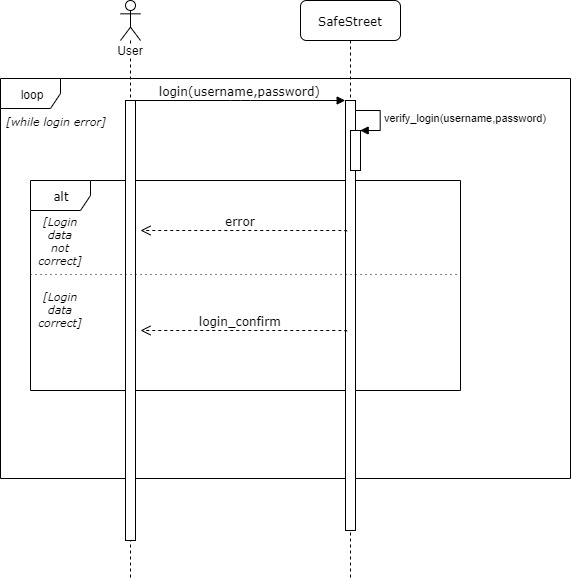
\includegraphics[width=\textwidth]{SequenceUserLogin}
\caption{Sequence diagram for \hyperref[uc:1]{use case n.1 ((User logs in)} }
\label{fig:seq-userlogin}
\end{figure}

\begin{figure}[htp]
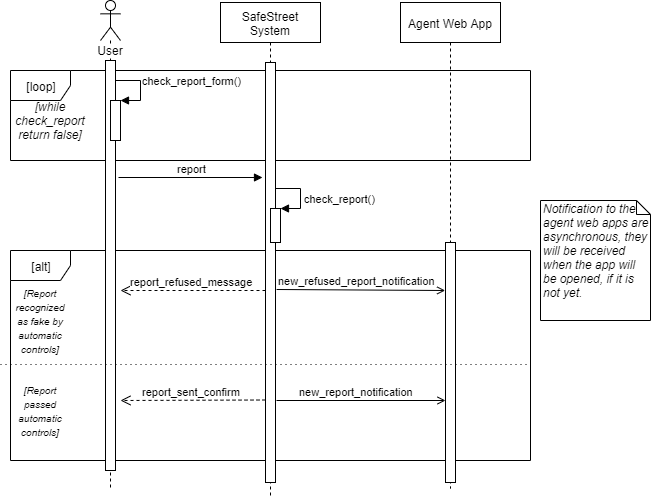
\includegraphics[width=\textwidth]{SequenceSendReport}
\caption{Sequence diagram for \hyperref[uc:2]{use case n.2 (User reports a violation)} }
\label{fig:seq-userreport}
\end{figure}

\begin{figure}[htp]
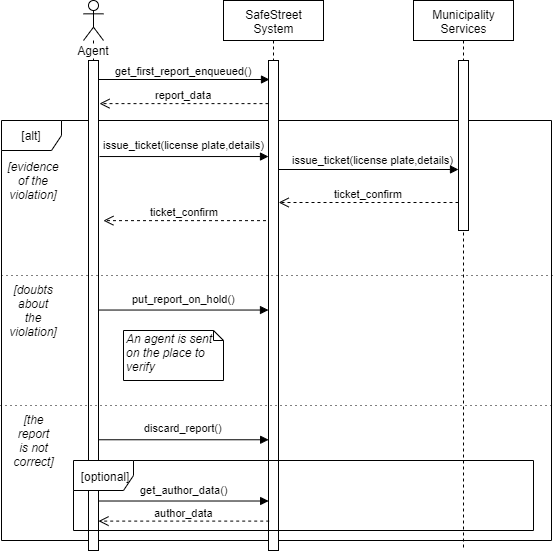
\includegraphics[width=\textwidth]{SequenceAgentCheckReport}
\caption{Sequence diagram for \hyperref[uc:7]{use case n.7 (Agents checks a notified violation)} }
\label{fig:seq-agentcheckreport}
\end{figure}

\begin{figure}[htp]
\centering
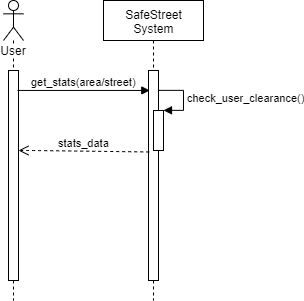
\includegraphics[scale=0.7]{SequenceCheckStatistics}
\caption{Sequence diagram for \hyperref[uc:5]{use case n.5 (Checking statistics)} }
\label{fig:seq-checkstats}
\end{figure}



\section{External interface requirements}
\subsection{User Interfaces}
In figures \ref{fig:mock-webreports} and \ref{fig:mock-suggestions} are provided some mockups of the user interfaces for the main functions of the system. They are just an approximate idea of how they should appear.
\begin{figure}
\begin{minipage}{.45\textwidth}
\centering
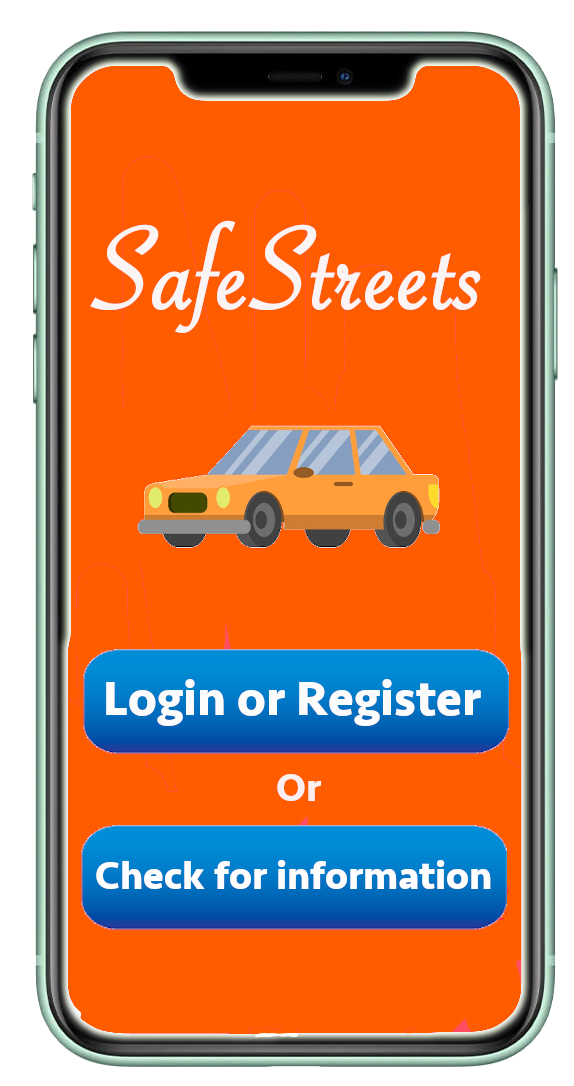
\includegraphics[width=.7\linewidth]{mockups/phoneschermatainiziale.png}
\caption[Mobile App mockup for initial page]{Mobile App mockup for the starting page after having opened the app for a User}
\label{fig:initial-page}
\end{minipage}\hfill
\begin{minipage}{.45\textwidth}
\centering
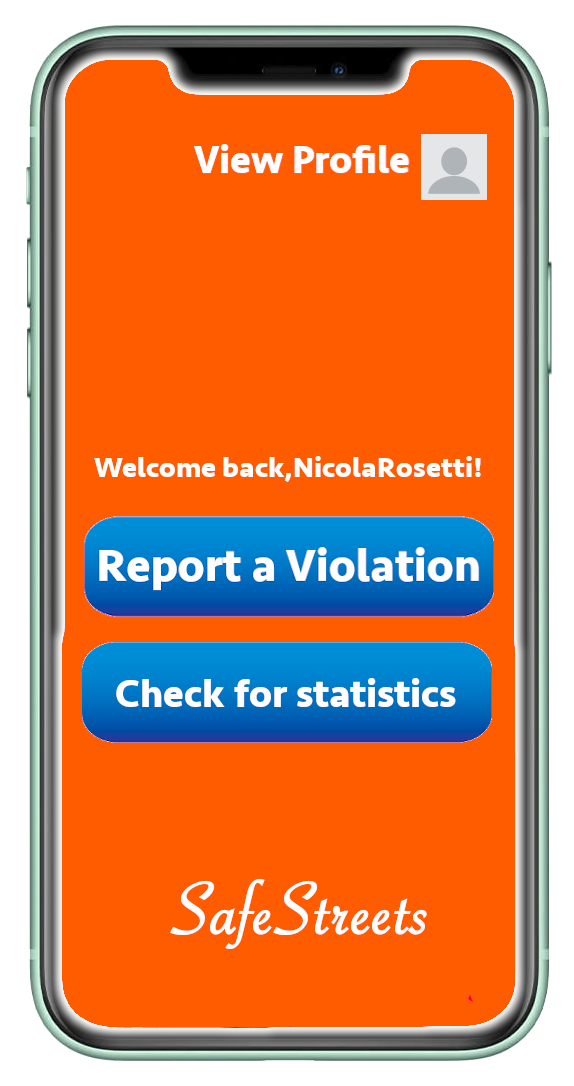
\includegraphics[width=.7\linewidth]{mockups/Schermata_principale.png}
\caption[Mobile App mockup for main page]{Mobile App mockup for the main page of the application after a User has logged in }
\label{fig:main-screen}
\end{minipage}
\end{figure}
\begin{figure}
\begin{minipage}{.45\textwidth}
\centering
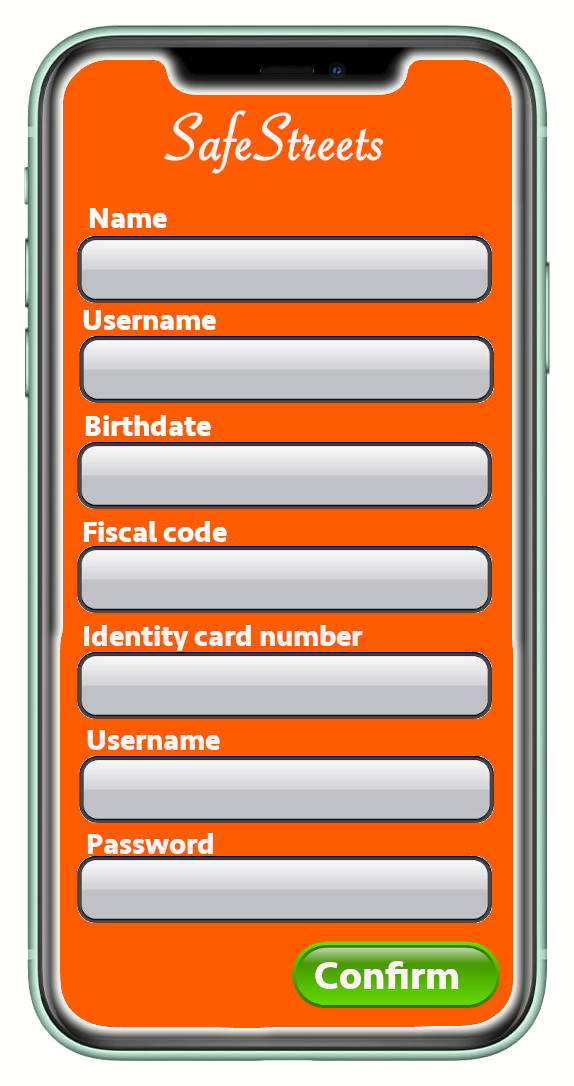
\includegraphics[width=.7\linewidth]{mockups/Register.png}
\caption[Mobile App mockup for the registration]{Mobile App mockup for a User when he wants to register}
\label{fig:register-page}
\end{minipage}\hfill
\begin{minipage}{.45\textwidth}
\centering
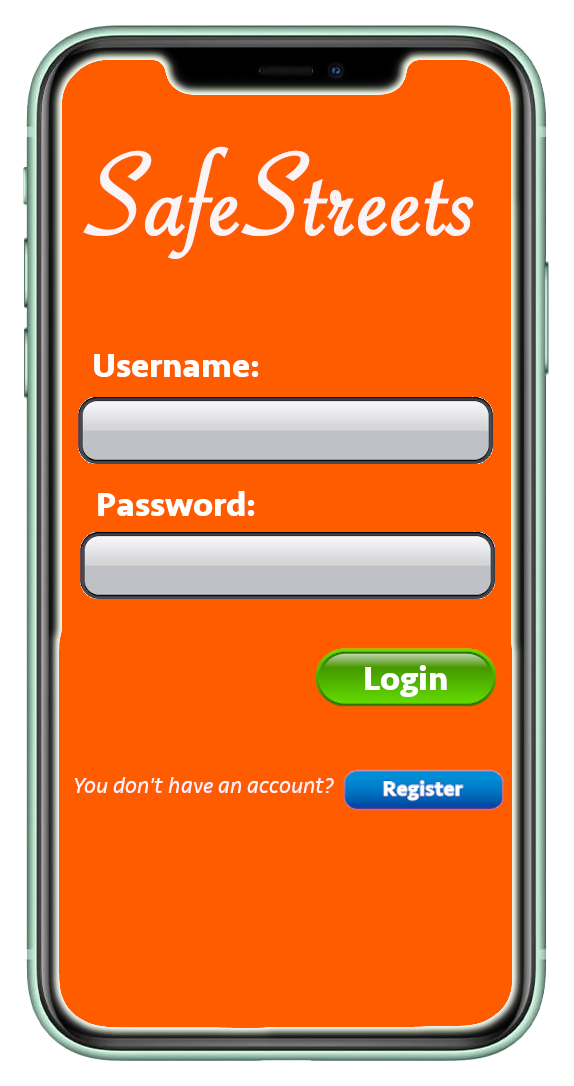
\includegraphics[width=.7\linewidth]{mockups/loginscreen.png}
\caption[Mobile App mockup for the login screen]{Mobile App mockup interface for the login of a registered User}
\label{fig:login-page}
\end{minipage}
\end{figure}
\begin{figure}
\begin{minipage}{.45\textwidth}
\centering
\includegraphics[width=.7\linewidth]{mockups/Report.png}
\caption[Mobile App mockup for the report page]{Mobile App interface mockup for the reporting of a violation for registered Users}
\label{fig:report-page}
\end{minipage}\hfill
\begin{minipage}{.45\textwidth}
\centering
\includegraphics[width=.7\linewidth]{mockups/Checkstatistics.png}
\caption[Mobile App mockup for statistics]{Mobile App interface mockup for the statistics for Users}
\label{fig:check-statistics}
\end{minipage}
\end{figure}
\begin{figure}[htp]
\centering
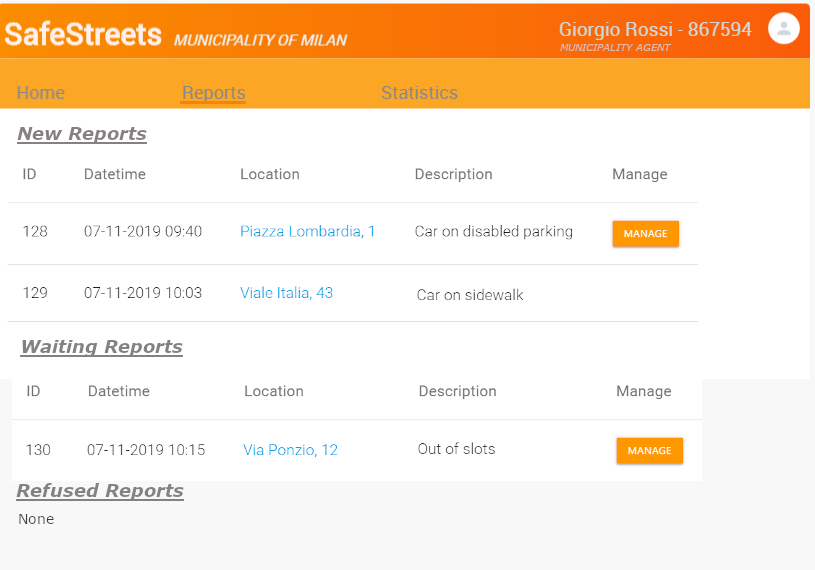
\includegraphics[width= \textwidth]{mockups/homeReport.png}
\caption[Web mockup for reports page]{Web interface mockup for the report list for a logged Municipality Agent }
\label{fig:mock-webreports}
\end{figure}
\begin{figure}[htp]
\centering
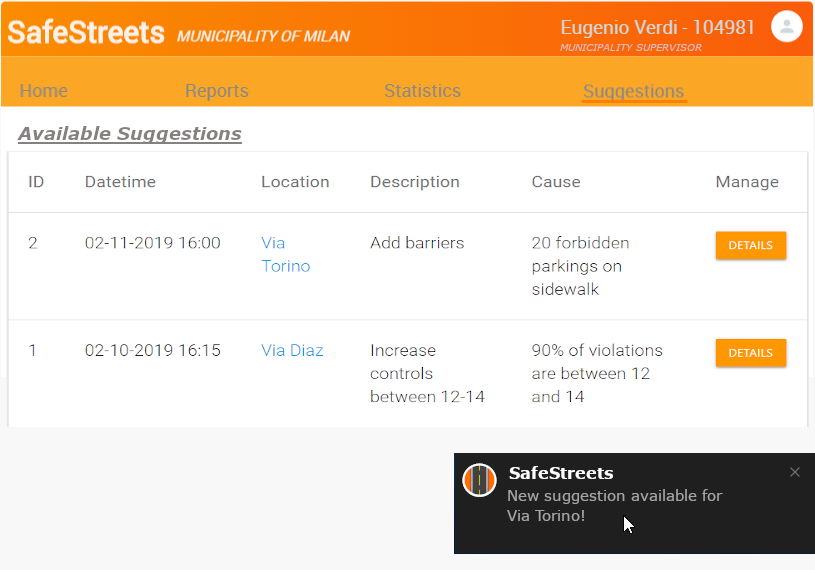
\includegraphics[width= \textwidth]{mockups/homeSuggestions.png}
\caption[Web mockup for suggestions page]{Web interface mockup for the suggestions list for a logged Municipality Supervisor}
\label{fig:mock-suggestions}
\end{figure}
\subsection{Hardware Interfaces}
No hardware interfaces are provided, being SafeStreets just a software system.
\subsection{Software Interfaces}
The system does not provide any software interface, because there are no other application which actually need to retrieve data from it. \\
The system has to call the municipalities services to retrieve some information (see \ref{SS-Dep&Const} ).
\subsection{Communication Interfaces}
The communication between users and SafeStreets servers exploit internal APIs through the \textit{HTTPS} protocol. The same is assumed for the communication with the municipalities systems. \\
For the \textit{users} the communication is unidirectional, in the sense that they cannot receive requests/notification by the server, all communications start from them. \\
The \textit{municipality agents} can be notified from the server when there are new report to be analyzed. \\
The \textit{municipality supervisors} can be notified about suggestions for interventions on the most unsafe areas.

\section{Functional requirements}
\label{sec:fun-requirements} 
For each goal we describe here the necessary functional requirements, which guarantee its satisfaction together with the domain assumptions:
\begin{itemize}
\item \hyperref[G1]{[G1]} People must be allow to report parking violations (missing parking disk, not paid parking meter, illegally parked vehicles).
\begin{itemize}
\item {[R1]}	\label{R1}The system must allow people to register to it providing personal data (name, surname, birthdate, identity card number, fiscal code) and selecting a username and a password.
\phantomsection
\item {[R2]}	\label{R2}The system must verify the correctness of the provided personal data of a registered user checking them from the identity card number, blocking the registration if they are not correct.
\item {[R3]}	\label{R3}The system must allow registered users to login through their username and password.
\item {[R4]}	\label{R4}The system must allow logged user to fill a report violation form.
\item {[R5]}	\label{R5}The system must let the user select the type of violation detected.
\item {[R6]}	\label{R6}The system must allow the user to insert the license plate in a violation report.
\item {[R7]}	\label{R7}While reporting the violation, the system must allow users to take one or more pictures of the potential violation.
\item {[R8]}	\label{R8}The system must not allow users to choose pictures not taken in the moment of the report.
\item {[R9]}	\label{R9}The system must collect the current position of the user, using GPS.
\item {[R10]}	\label{R10}The system must allow user to confirm or delete the current report.
\item {[R11]}	\label{R11}After confirmation, the system must add the current date and time to the report.
\item {[R12]}	\label{R12}The system must store confirmed report.
\end{itemize}
\item \hyperref[G2]{[G2]} Municipality agents must be notified about reports of potential violations in their area of interest, which can be possibly used to generate traffic tickets.	
\begin{itemize}
\item {[R13]}	\label{R13}The system must check reports to try to find if the pictures of the violations have been modified.
\item {[R14]}	\label{R14}The system must try to find, according to the GPS position of the user and the pictures sent, if the position is fake or not.
\item {[R15]}	\label{R15}The system must discard the report if it has been recognized as fake according to the previous requirements (R13-R14).
\item {[R16]}	\label{R16}The system must try to automatically recognize the license plate in the photo, possibly with the help of the value inserted by the user.
\item {[R17]}	\label{R17}The system must store into stable memory the reported violation if correct (i.e. not recognized as fake).
\item {[R18]}	\label{R18}The involved municipality must be calculated considering in which city the reported violation has been found, based on the GPS position of the user that has sent the report.
\item {[R19]}	\label{R19}The system must send the reported violations to the involved municipality.
\item {[R20]}   \label{R20}The system must allow an agent to see the reports for its municipality, checking them in order of arrival
\item {[R21]}	\label{R21}The system must allow an agent to issue a traffic ticket to a certain person (i.e. license plate) through the correspondent municipality service.
\item {[R22]}	\label{R22}The system must allow an agent to put on hold a violation report if it needs to be checked in person.
\item {[R23]}	\label{R23}\label{R20}The system must allow an agent to discard a violation if it has been verified as fake or it cannot be verified (the vehicle is not there anymore) or it is a duplicated report.
\item {[R24]}	\label{R24}The system must allow an agent to retrieve the data of the author of a violation report.
\phantomsection
\item {[R25]}	\label{R25}The system must allow an agent to create an account, asking the municipality services to verify its identity.
\item {[R26]}	\label{R26}The system must allow an agent to login, inserting its username and password.
\end{itemize}
\item  \hyperref[G3]{[G3]} People must be allowed to retrieve information about streets or areas with the highest frequency of violations.
\begin{itemize}
\item {[R27]}	\label{R27}The system must mine this information from the reported violations.
\item {[R28]}	\label{R28}The system must allow the users (even if not authenticated) to select the see information for a city. The user can choose either the city where he is, using the GPS position, or an arbitrary selected location.
\item {[R29]}	\label{R29}The system must allow the user to select information about streets or areas in the city selected and to specify if he wants information for a specific street or area or a classification of streets or areas.
\item {[R30]}	\label{R30}The system must show the the data corresponding to the selection of [R29]
\end{itemize}
\item  \hyperref[G4]{[G4]} People must be able to retrieve statistics and trends about the accidents correlated to the parking violations, the effectiveness of SafeStreets initiatives and the issuing of traffic tickets.
\begin{itemize}
\item {[R31]}	\label{R31}The system must take information about accidents and tickets from the municipality.
\item {[R32]}	\label{R32}The system must use this information to build statistics, crossing them with reported violations.
\item {[R33]}	\label{R33}The system must not allow common users to see confidential data about other people.
\item {[R34]}	\label{R34}The system must allow the user to choose a topic: areas or streets with most accidents, areas or streets with the highest number of traffic tickets issued, areas or streets where there have been the best improvements, information for a specific area or street.
\item {[R35]}	\label{R35}The system must show to the user the information about the topic selected according to [R34].
\end{itemize}
\item  \hyperref[G5]{[G5]} Municipality supervisors must be able to retrieve data about the vehicles with the highest number of violations.
\begin{itemize}
\item {[R36]}	\label{R36}The system must allow authenticated supervisors to retrieve information about the vehicles with the highest number of violations in a selected area or street.
%\item {[R37]}	\label{R37}The system must allow supervisors to see what areas or streets has seen the best improvements in the ticket emissions.
\item {[R37]}	\label{R37}The system must allow supervisors to access only information about their own municipality.
\item {[R38]}	\label{R38}The system must allow a supervisor to create an account, asking the municipality services to verify its identity.
\item {[R39]}	\label{R39}The system must allow a supervisor to login, inserting its username and password.
\end{itemize}
\item  \hyperref[G6]{[G6]} Municipalities must be suggested for possible interventions about the mostly unsafe areas.
\begin{itemize}
\item {[R40]}	\label{R40}The system must take information about accidents, tickets and street networks (bike lanes, sidewalks, parking areas,…) from the municipality, exploiting the municipality services.
\phantomsection
\item {[R41]}	\label{R41}The system must elaborate this information, combined with reports information, and try to find possible solutions for problems.
\item {[R42]}	\label{R42}The system must notify the municipality supervisors about the solutions it has found.
\end{itemize}
\end{itemize}


\section{Performance requirements}
Performance requirements are not particularly critical for the system, but it is anyway desirable that all requests sent to the server are answered within 1 second, to assure a good user experience. \\
The server infrastructure will be designed to be scalable so that it will be possible to adapt it to the increment of users when the app diffusion will increase.
\section{Design constraints}
%\subsection{Standards compliance}
\subsection{Regulatory policies}
The application will only record the data strictly correlated to the reported violations and the data provided by the users during the registration. This data will be used only for the purposes of the system and will be treated confidentially, according to the \textit{GPDR} rules.\\
In particular the statistical analyses performed will never show publicly any information which can be related to a specific person.
\subsection{Hardware and software limitations}
The following requirements are necessary to install the mobile application:
\begin{itemize}
\item \textit{Operating system}: Android 5+ or iOS 9+
\item \textit{Hardware}: to allow the access as logged user the smartphone needs to have a camera and a GPS sensor
\end{itemize}
The camera is needed to take photos of the violations and the GPS is necessary to automatically record the position. The users have to give the relative permissions to the application. A base necessary requirement to use any functionality is the presence of an internet connection.\\
This requirements allow the majority of people to use the application \label{use:os-stats}  \mbox{(see \hyperref[ref:os-stats]{\textit{[OS-STAT]}}).}\\
The authorities have the possibility to use a web interface, accessible through every modern browser.\\
Everyone can consult the publicly available statistics also through the \textit{SafeStreets website}, with any modern browser.
%\subsection{Any other constraints}
%//PROBABLY NOTHING
\section{Software system attributes}
\subsection{Availability}
The availability is not a critical requirement, but the system has to guarantee a 99\% of uptime (max 3.65 days/year of downtime) to ensure that the users can normally use it.
\subsection{Security}
Security is a critical requirement for this system, considering the confidential information that are transmitted through it. It is assured by the use of the \textit{HTTPS} protocol for all communications and by the follow of the best security practices for the servers management, protecting them with IDS, maintaining the data ciphered and assuring the access only to the authorized users. \\
Every activity performed by municipality agents and supervisors will be logged to ensure its traceability.
\subsection{Maintainability}
The system will be realized following the best software engineering practices to ensure its maintainability and expandability in the future.
\subsection{Portability}
The system is actually designed to be compatible with most of Android and iOS devices (smartphones and tablets) and from the authorities side it can be accessed from any web browser, so it is very portable.
It will be important to maintain it compatible with the future releases of this two operating systems and with any other new operating system or device that will acquire an important market share.
\chapter{Formal Analysis using Alloy}
\section{Introduction}
In this section is shown a formal analysis of some aspects of the system using Alloy. The main purpose of this analysis is to formally define the constraints which allow the system to work properly, both external constraints (i.e. domain assumptions) and internal constraints (i.e. requirements). \\
The signatures defined do not have an exact correspondence with the classes of the Class Diagram (see \ref{fig:class-diagram}), even if there is a good matching. The main differences are the absence of some fields or classes which are not useful for this modeling activity and the presence of some signatures (\textit{StatisticsRequest} and the related \textit{StatisticsLevel} and \textit{RequestStatus}) which do not have correspondent classes in the previously shown uml diagram. This is due to the fact that they are technical classes, not necessary to be shown in the general abstract class diagram, whose purpose is just to show the domain of the application, but it can be useful to have them here as signatures to allow to express a particular constraint (i.e. the privacy levels of statistics data). There are some simplifications, in particular the use of the Alloy built-in type \textit{Time} which easy allows to define time instants and check their order, but clearly does not have the same expressive power of a \textit{DateTime} type of a high-level programming language.\\
This Alloy model manly consists of signatures and facts. A summary of what is expressed through the facts and a matching with the previously expressed requirements and domain assumptions (see \ref{sec:fun-requirements} and \ref{subsec:domain-ass}) is the following:
\begin{itemize}
\item Every area has at least one city and every street can be only in areas of the same municipality \hyperref[D3]{[D3]}
\item The state evolution of a \textit{Report} is consistent with the StateDiagram (\ref{fig:state-diagram1}), every report is checked by a municipality agent of the same municipality where the violation has occurred \hyperref[R15]{[R15-22]}
\item Every \textit{StatisticsData} is referred to an area or to a street, but not both \hyperref[R29]{[R29]}
\item The are no users with the same identity card number, fiscal code or username \hyperref[R2]{[R2]}
\item Every municipality has at least one street [the concept of Municipality impose this]
\item Agents must check the reports in the order of emission \hyperref[R20]{[R20]}
\item An agents cannot issue traffic tickets in another city \hyperref[R19]{[R19, R21]}
\item For every approved report there is a correspondent ticket \hyperref[R21]{[R21]}
\item For every street where there have been at least two accidents caused by bad parked cars and two approved reports there must be a suggestion. This is an easy example to answer the requirement \hyperref[R41]{[R41]}
\item \textit{ReservedStatistics} can be accessed only by Supervisors \hyperref[R33]{[R33]}
\item Correctness of statistics data \hyperref[R29]{[R29,R30,R34,R35,R36]}
\end{itemize}
This model does not easy allow to express assertions to be checked, because it already covers almost all about the requirements/assumptions which involves and there are no very interesting and non trivial properties which should be implied by it and so should be checked through assertions. The goals of system, which are what is really implicated by the combination of requirements and assumptions, cannot be easily expressed in a "machine" formal way, without falling in a repetition of the requirements. Anyway there are a pair of assertions which state that the number of approved reports must be smaller or equal to the number of the tickets, for all agents and for all streets. This clearly follows by the fact that every approved reports has a consequent ticket and it's not a simple equality because the municipality can issue other tickets, not associated to reports, but still in the application data thanks to the information collected from the municipality for statistics elaboration.\\
At the end of the Alloy code there are some predicates which are then shown and explained.\\
The predicates are consistent and no counterexample has been found for the assertions, by the tool:
\begin{figure}[hp]
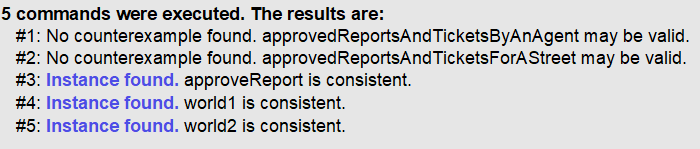
\includegraphics[width=\textwidth]{alloyResults}
\caption{Alloy tool validation results}
\label{fig:alloyResults}
\end{figure}

\section{Alloy code}
\lstinputlisting[language=alloy]{alloyModel.als}

\section{Generated worlds}
The predicate \textit{world1} generates a first world (figure \ref{fig:world1}) which shows the presence of a \textit{Suggestion} as a consequence of the two \textit{Approved} \textit{Reports} and the two \textit{Accidents} caused by \textit{BadParkedCars} in the unique \textit{Street} of the world, all over two consecutive time instants (not shown in figure, the diagram is projected over time for better readability). It can also be observed the presence of the two \textit{Tickets} associated to the two \textit{Approved Reports} and the correspondence of \textit{MunicipalityAgents} for \textit{Tickets} and relative \textit{Reports}.\\
The second one (figure \ref{fig:world2} ) shows Statistics information which are coherent with the tickets, reports and accidents data (it's still projected over Time, but it can be seen that all events happen at the same time). \\
Finally the predicate \textit{ApproveReport} (figure \ref{fig:approveReport}) shows the change of state of a Report which becomes \textit{Approved}, showing the consistency of the state evolution and the corresponding \textit{Ticket} generated.

\newgeometry{bottom=2cm}
\begin{landscape}

\begin{figure}[hp]
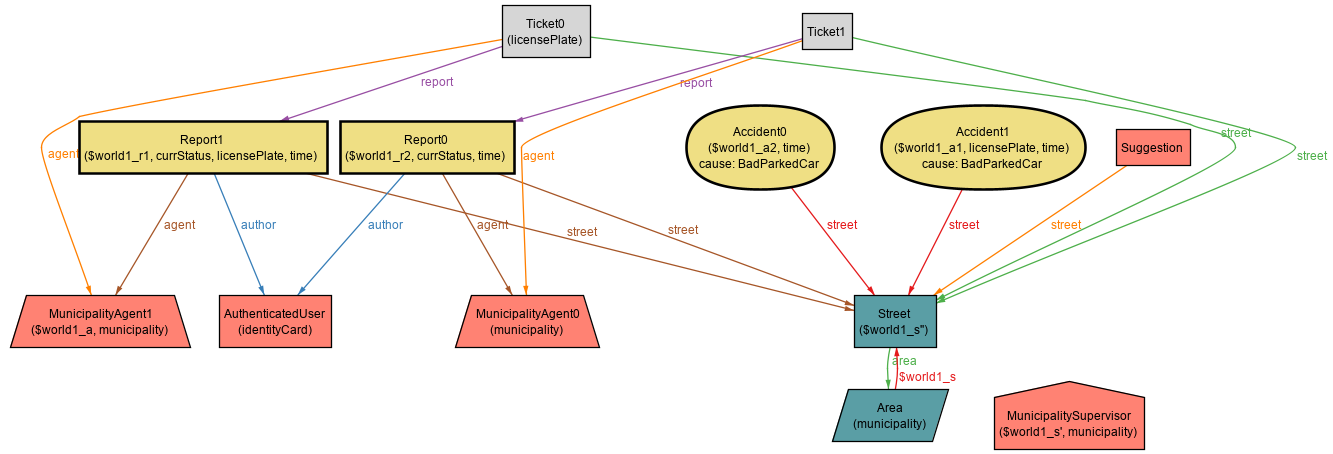
\includegraphics[angle=0, scale=0.55]{world1}
\caption{Alloy World n.1}
\label{fig:world1}
\end{figure}
\end{landscape}

\begin{landscape}
\begin{figure}[hp]
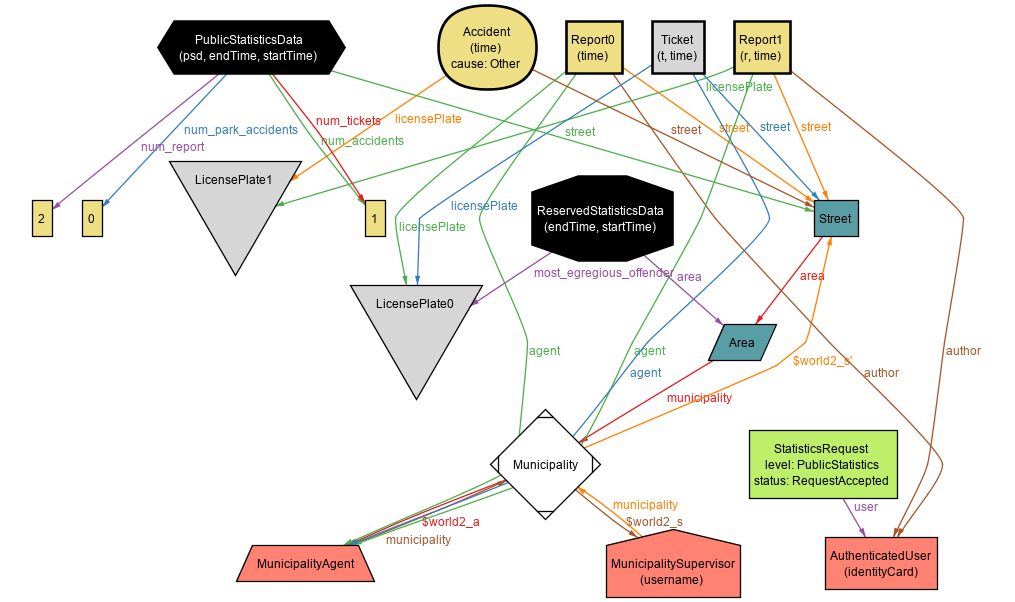
\includegraphics[angle=0, scale = 0.7]{world2-2}
\caption{Alloy World n.2}
\label{fig:world2}
\end{figure}
\end{landscape}

\begin{landscape}
\begin{figure}[hp]
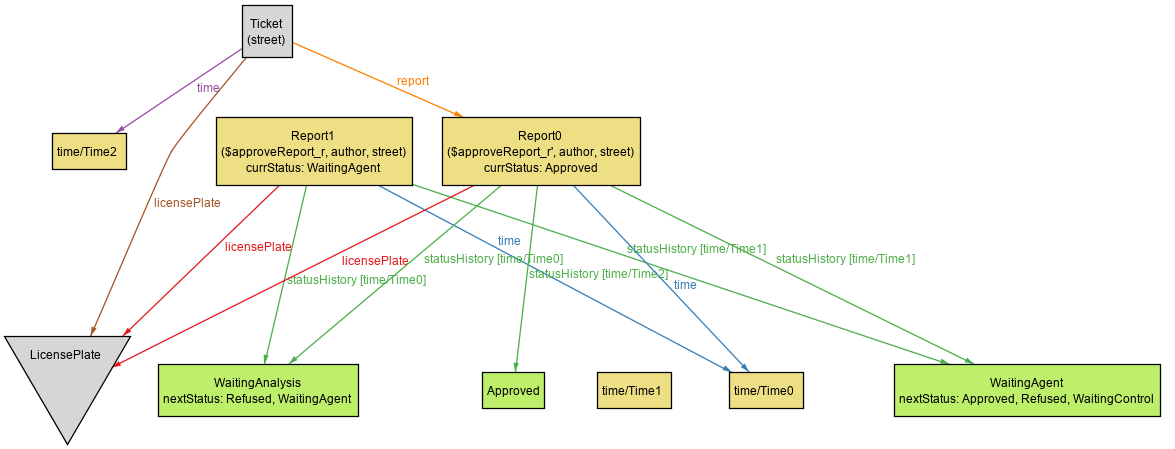
\includegraphics[angle=0, scale=0.6]{reportApprovation}
\caption{Alloy predicate ApproveReport}
\label{fig:approveReport}
\end{figure}
\end{landscape}


\restoregeometry

\chapter{Effort spent}

\begin{table}[H]
\centering
Nicola Rosetti \\
%\begin{tabular}{lll}
\begin{tabular}{p{2cm}p{1.5cm}p{7cm}}
\toprule
\textit{Date} & \textit{Hour} & \textit{Section} \\ \midrule
17-10-2019 & 1.5 h* & Goals \\ \midrule
19-10-2019 & 3.5 h & Goals revision and requirements outline  \\ \midrule
20-10-2019 & 1 h & Goals and requirements revision \\ \midrule
22-10-2019 & 2 h & Scenarios \\ \midrule
23-10-2019 & 2 h & Product functions \\ \midrule
24-10-2019 & 2 h & Scenarios \\ \midrule
26-10-2019 & 1.5 h & Use Cases writing \\ \midrule
29-10-2019 & 2 h & Use Case revision\\ \midrule
31-10-2019 & 1 h & Scenario and use cases transcription \\ \midrule
31-10-2019 & 0.5 & Introduction, revision on domain assumptions and transcription of them on the RASD \\ \midrule
31-10-2019 & 1 h* & Alloy \\ \midrule
3-11-1019 & 2h & Mockups\\ \midrule
4-11-1019 & 2h & Mockups\\ \midrule
5-11-1019 & 2h & Mockups\\ \midrule
6-11-1019 & 2h & Mockups\\ \midrule
8-11-1019 & 2h & Mockups\\ \midrule
10-11-2019 & 2 h & Last Mockups and Mockup insertion in RASD \\
\bottomrule
\end{tabular}
\caption[Nicola Rosetti's effort table]{}
\end{table}


\vspace*{1 cm}
\begin{table}[H]
\centering
Simone Sartoni \\
\begin{tabular}{p{2cm}p{1.5cm}p{7cm}}
\toprule
\textit{Date} & \textit{Hour} & \textit{Section} \\ \midrule
17-10-2019 & 1.5 h* & Goals \\ \midrule
20-10-2019 & 4.5 h & Goals revision and requirements outline  \\ \midrule
22-10-2019 & 3 h & Goals and requirements revision \\ \midrule
23-10-2019 & 1.5 h & Use Case UML model design and draw \\ \midrule
24-10-2019 & 2 h & Goal and requirements revision, functions \\ \midrule
25-10-2019 & 2 h & Use Case UML model update \\ \midrule
27-10-2019 & 1.5 h & Use Cases writing \\ \midrule
29-10-2019 & 2 h & Use Case UML model and use cases revision \\ \midrule
31-10-2019 & 1 h & Scenario and use cases revision \\ \midrule
04-11-2019 & 1.5 h & Goals transcription on the RASD \\ \midrule
05-11-2019 & 2.5 h & Requirements transcription on the RASD \\ \midrule
07-11-2019 & 1.5 h & Title page disposition \\ \midrule
08-11-2019 & 1 h & Title page update \\
\bottomrule
\end{tabular}
\caption[Simone Sartoni's effort table]{}
\end{table}
\vspace*{1 cm}
\begin{table}[H]
\centering
Vittorio Torri \\
\begin{tabular}{p{2cm}p{1.5cm}p{7cm}}
\toprule
\textit{Date} & \textit{Hour} & \textit{Section} \\ \midrule
17-10-2019 & 1.5 h* & Goals \\ \midrule
20-10-2019 & 1 h & Users, Hardware and software limitations, goal refinement \\ \midrule
21-10-2019 & 1 h & Software, Hardware and Communication Interfaces, Performance requirements, Design constraints, Software system attributes \\ \midrule
22-10-2019 & 1 h & Goal and requirements revision \\ \midrule
23-10-2019 & 1 h & Goal and requirements revision \\ \midrule
26-10-2019 & 2 h & Scenarios, requirements, functions, scope \\  \midrule
28-10-2019 & 1.5 h & Product perspective and UML Class Diagram \\ \midrule
29-10-2019 & 1 h & State diagram and sequence diagram \\ \midrule
31-10-2019 & 0.5 h & Sequence diagram \\ \midrule
31-10-2019 & 1 h* & Alloy \\ \midrule
02-11-2019 & 1.5 h & Sequence diagrams \& minor fixes \\ \midrule
03-11-2019 & 4 h & Alloy \\ \midrule
04-11-2019 & 1 h & Alloy \\ \midrule 
05-11-2019 & 1.5 h & Alloy \\ \midrule
06-11-2019 & 1.5 h & Alloy \\ \midrule
07-11-2019 & 1h & General revision \\ \midrule
08-11-2019 & 2h & General revision \\ \midrule
08-11-2019 & 2h & Alloy \\ \midrule
08-11-2019 & 2h & Web interface mockup (report list) \\ \midrule
09-11-2019 & 1h & Web interface mockup (suggestion list) \\ \midrule
09-11-2019 & 2h & General revision, tables 1.1 and 3.1\\ \midrule
10-11-2019 & 0.5h & Graphic corrections\\
\bottomrule
\end{tabular}
\caption[Vittorio Torri's effort table]{}
\end{table}
\textit{* Group work}

\chapter{References}
\begin{itemize}

\item \label{ref:os-stats} \hyperref[use:os-stats]{\textit{[OS-STAT]}} \href{https://gs.statcounter.com}{\textit{https://gs.statcounter.com}} - statistics on operating systems market share and versions diffusion

\item \label{ref:slander} \hyperref[use:slander]{\textit{[SLANDER]}} see art. 368, 370 and 69 c.p.p. (Italian law)

\end{itemize}

\end{document}
